\section{连续型随机变量的概率分布}

\subsection{连续型随机变量概率密度}

\begin{definition}[连续型随机变量概率密度]
    设随机变量 $ X $ 的分布函数是 $ F(x) $, 若存在一个非负可积函数 $ f(x) $, 使对于任意实数 $ x $, 都有
    $$F(x)=\int_{-\infty}^{x} f(t) \dd t ~(x \in \mathbb{R})$$
    则称 $ X $ 为连续型随机变量, 称 $ f(x) $ 为 $ X $ 的概率密度函数, 简称概率密度, 记为 $ X \sim f(x) .$
\end{definition}

\begin{theorem}[连续型随机变量概率密度的性质]
    概率密度 $ f(x) $ 的性质如下:
    \begin{enumerate}[label=(\arabic{*})]
        \item 非负性: $ f(x) \geqslant 0 $;
        \item 规范性: $ \displaystyle\int_{-\infty}^{+\infty} f(x) \mathrm{d} x=1$ ;
        \item 对任意实数 $ a \leqslant b$ 都有 $\displaystyle P\{a<X \leqslant b\}=\int_{a}^{b} f(x) \mathrm{d} x $;
        \item 若 $ f(x) $ 在点 $ x $ 处连续, 则有 $ F^{\prime}(x)=f(x) .$
    \end{enumerate}
\end{theorem}

设 $ X $ 是连续型随机变量, 已知其概率密度 $ f_{X}(x) $, 则由函数 $ y=g(x) $ 确定的随机变量 $ Y $ 可能是离散型随机变量, 也可能是连续型随机变量. \\
以连续为例, 求随机变量 $ Y $ 的分布函数 $ F_{Y}(y) $.
\begin{enumerate}[label=(\arabic{*})]
    \item 定义法: $\displaystyle F_{Y}(y)=P\{Y \leqslant y\}  =P\{g(X) \leqslant y\}  =\int_{g(x) \leqslant y} f_{X}(x) \mathrm{d} x$, 做题步骤:
          \begin{enumerate}
              \item 画出 $ y=g(x) $ 在 $ f(x) $ 正概率区间的图像;
              \item 找出 $ y=g(x) $ 在 $ y=y $ (动直线) 以下的图像, 确定该部分 $ x $ 的范围, 并用 $ y $ 表示;
              \item 求出 $ F_{Y}(y) $.
          \end{enumerate}
          若求连续型随机变量 $ Y $ 的概率密度 $ f_{Y}(y) $, 则分布函数 $ F_{Y}(y) $ 对 $ y $ 求导即可.
          $$
              f_Y(y)=\begin{cases}
                  \dfrac{\mathrm{d} F_{Y}(y)}{\mathrm{d} y}, & \text { 当 } F_{Y}(y) \text { 在 } y \text { 处可导时 }   \\
                  0,                                         & \text { 当 } F_{Y}(y) \text { 在 } y \text { 处不可导时 }
              \end{cases}
          $$
    \item 公式法: 若函数 $ y=g(x) $ 处处可导且严格单调 (恒有 $ g^{\prime}(x)>0 $ 或 $ g^{\prime}(x)<0)$, $ h(y) $ 为 $ g(x) $的反函数, 则 $ Y=g(X) $ 是连续型随机变量,
          其概率密度为
          $$
              f_{Y}(y)=\begin{cases}
                  f_{X}[h(y)]\left|h^{\prime}(y)\right|, & \alpha<y<\beta \\
                  0,                                     & \text { 其他 }
              \end{cases}
          $$
          其中 $ (\alpha, \beta) $ 为函数 $ y=g(x) $ 的值域.
\end{enumerate}

\begin{theorem}
    在任何点取值的概率均为 0 的随机变量为连续型随机变量.
\end{theorem}

\subsection{均匀分布}

\begin{definition}[均匀分布]
    若随机变量 $ X $ 的概率密度为
    $$f(x)=\begin{cases}
            \dfrac{1}{b-a}, & a<x<b           \\[6pt]
            0,              & \text { 其他 .}
        \end{cases}$$
    则称 $ X $ 在区间 $ (a, b)$ 上服从均匀分布, 记为 $ X \sim U(a, b) $.
    其分布函数为
    $$F(x)=\begin{cases}
            0,                & x<a             \\
            \dfrac{x-a}{b-a}, & a \leqslant x<b \\[6pt]
            1,                & b \leqslant x.
        \end{cases}$$
\end{definition}

\subsection{指数分布}

\begin{definition}[指数分布]
    若随机变量 $ X $ 的概率密度为
    $$f(x)=\begin{cases}
            \lambda \mathrm{e}^{-\lambda x}, & x>0           \\
            0,                               & x \leqslant 0
        \end{cases}$$
    则称 $ X $ \textit{服从参数为} $ \lambda(\lambda>0) $ \textit{的指数分布}, 记为 $ X \sim E(\lambda) $, 其分布函数为
    $$F(x)=\begin{cases}
            1-\mathrm{e}^{-\lambda x}, & x>0           \\
            0,                         & x \leqslant 0
        \end{cases}$$
    \begin{enumerate}[label=(\arabic{*})]
        \item 指数分布常用来描述电子元器件的寿命, $P\{X>x\}=\mathrm{e}^{-\lambda x} $;
        \item 指数分布具有无记忆性, 对于任意 $ s, t>0$, 有 $P\{X>s+t \mid X>s\}=P\{X>t\} .$
    \end{enumerate}
    \index{指数分布}
\end{definition}

\begin{example}
    设随机变量 $X$ 服从参数为 $1$ 的指数分布, 求 $P\qty{3>X>2|X>1}$.
\end{example}
\begin{solution}
    $\displaystyle P\qty{3>X>2|X>1}=P\qty{X>2|X>1}-P\qty{X>3|X>1}=P\qty{X>1}-P\qty{X>2}=\int_{1}^{+\infty} \e ^{-x} \dd x-\int_{2}^{+\infty} \e ^{-x} \dd x=\e ^{-1}-\e ^{-2}.$
\end{solution}

\begin{example}
    设 $X$ 是服从参数为 2 的指数分布的随机变量, 求随机变量 $Y=X-\dfrac{1}{2}$ 的概率密度函数 $f_Y(y).$
\end{example}
\begin{solution}
    因为 $X\sim E(2)$, 所以其概率密度为 $f_X(x)=\begin{cases}
            2\e^{-2x}, & x>0          \\
            0,         & x\leqslant 0
        \end{cases}$, 现 $Y+x-\dfrac{1}{2}$, 所以 $$F_Y(y)=P\qty{Y\leqslant y}=P\qty{X-\dfrac{1}{2}\leqslant y}=P\qty{X\leqslant y+\dfrac{1}{2}}=\int_{-\infty}^{y+\frac{1}{2}}f_X(x)\dd x=F_X\qty(y+\dfrac{1}{2})$$
    那么 $$f_Y(y)=F'_Y(y)=F'_X(x)\qty(y+\dfrac{1}{2})=f_X(y+\dfrac{1}{2})=\begin{cases}
            2\e^{-2y-1}, & y>-\dfrac{1}{2}          \\[6pt]
            0,           & y\leqslant -\dfrac{1}{2}
        \end{cases}$$
\end{solution}

\begin{example}
    设随机变量 $X\sim E(2)$, $a$ 为大于 2 的常数, 已知 $P\qty{X\leqslant a~|~X>2}=1-\e^{-2}$, 求 $a.$
\end{example}
\begin{solution}
    \textbf{法一: }因为 $P\qty{X\leqslant a~|~X>2}=1-P\qty{X>a~|~X>2}$, 于是
    \begin{flalign*}
        P\qty{X\leqslant a~|~X>2} & =1-\dfrac{P\qty{X>a,X>2}}{P\qty{X>2}}=1-\dfrac{P\qty{X>a}}{P\qty{X>2}}=1-\dfrac{\displaystyle\int_{a}^{+\infty}2\e^{-2t}\dd t}{\displaystyle\int_{2}^{+\infty}2\e^{-2t}\dd t} \\
                                  & =1-\dfrac{\e^{-2a}}{\e^{-4}}=1-\e^{-2(a-2)}=1-\e^{-2}.
    \end{flalign*}
    解得 $a=3.$\\
    \textbf{法二: }$P\qty{X\leqslant a~|~X>2}=1-P\qty{X>a~|~X>2}=1-P\qty{X>a-2}=1-\e^{-2(a-2)}=1-\e^{-2}\Rightarrow a=3.$
\end{solution}

\begin{example}
    已知随机变量 $X\sim E(\lambda)~~(\lambda>0)$, 且随机变量 $Y=\begin{cases}
            X,  & |X|\leqslant 1 \\
            -X, & |X|> 1
        \end{cases}$, 求 $P\qty{Y\leqslant \dfrac{1}{2}}.$
\end{example}
\begin{solution}
    \begin{minipage}{0.29\linewidth}
        \begin{figure}[H]
            \centering
            \begin{tikzpicture}[->,samples=100,>=stealth,font=\footnotesize,scale=0.85]
                \draw[->,cyan](-2,0)--(0,0)node[below right]{$O$}--(2,0)node[below]{$X$};
                \draw[->,cyan](0,-4)--(0,2)node[left]{$Y$};
                \draw[densely dashed,-] (0,1)--(1,1)--(1,0)node[below right]{$1$};
                \draw[densely dashed,-,rotate=180] (0,1)--(1,1)--(1,0);
                \draw[-,black,domain=-1:1] plot({\x},{\x})node[right]{$Y=X$};
                \draw[fill=black] (1,1) circle (0.5pt);
                \draw[fill=black,rotate=180] (1,1) circle (0.5pt);
                \draw[-,black,domain=-1.5:-1] plot(\x,{-\x})node{$\circ$};
                \draw[-,black,domain=-1.5:-1,rotate=180] plot(\x,{-\x})node{$\circ$};
                \draw[-,densely dashed,black,domain=-1:1] plot(\x,{-\x});
                \draw[-,orange] (-1.5,0.5) -- (1.5,0.5)node[right]{$Y=\dfrac{1}{2}$};
                \draw[-,magenta,domain=-1.5:-1] plot(\x,{\x-2})node{$\circ$};
                \draw[-,black,domain=-1:0.5,densely dashed] plot(\x,{\x-2});
                \draw[-,magenta,domain=0.5:1,rotate=180,yshift=2.5cm,xshift=-1.5cm] plot(\x,{\x-2})node{$\circ$};
                \draw[-,densely dashed] (-1,-1)--(-1,-3);
                \draw[-,densely dashed] (0.5,0.5)--(0.5,-1.5);
            \end{tikzpicture}
            \caption{}
            \label{sjbldasd}
        \end{figure}
    \end{minipage}\hfill
    \begin{minipage}{0.7\linewidth}
        由图 \ref{sjbldasd} 可知,
        \begin{flalign*}
            P\qty{Y\leqslant \dfrac{1}{2}} & =P\qty{-1\leqslant X\leqslant \dfrac{1}{2}}+P\qty{X>1}            \\
                                           & =P\qty{-1\leqslant X\leqslant \dfrac{1}{2}}+1-P\qty{X\leqslant 1} \\
                                           & =1-P\qty{X<-1}+P\qty{\dfrac{1}{2}<X\leqslant 1}
        \end{flalign*}
        而 $P\qty{X<-1}=0$, 因此 $$P\qty{Y\leqslant \dfrac{1}{2}}=1-P\qty{\dfrac{1}{2}<X\leqslant 1}=1-\int_{\frac{1}{2}}^{1}\lambda\e^{-\lambda x}\dd x=1+\e^{-\lambda}-\e^{-\frac{\lambda}{2}}.$$
    \end{minipage}
\end{solution}

\subsection{正态分布}

\begin{definition}[正态分布及其分布函数]
    \label{normalDistributionAndItsDistributionFunction}
    \index{正态分布及其分布函数}
    若随机变量 $X$ 的密度为 $f(x)=\dfrac{1}{\sqrt{2\pi}\sigma}\e^{-\frac{(x-\mu)^2}{2\sigma^2}}$, 则称 $X$ 服从参数为 $\mu,~\sigma$ 的正态分布, 简记为 $X\sim N\qty(\mu,\sigma^2)$, $X$ 的分布函数为 $\displaystyle F(x)=\int_{-\infty}^{x}\dfrac{1}{\sqrt{2\pi}\sigma}\e^{-\frac{(t-\mu)^2}{2\sigma^2}}\dd t.$
\end{definition}

\begin{theorem}[对称性]
    \index{对称性}一般正态分布 $N\qty(\mu,\sigma^2)$ 的概率密度 $f(x)$ 满足 $f(x)=f(2\mu-x).$
\end{theorem}
\begin{theorem}[和一性]
    \index{和一性}一般正态分布 $N\qty(\mu,\sigma^2)$ 的分布函数 $F(x)$ 满足 $F(x)+F(2\mu-x)=1.$
\end{theorem}

\begin{definition}[标准正态分布]
    \index{标准正态分布}
    当定义 \ref{normalDistributionAndItsDistributionFunction} 中 $\mu=0,~\sigma=1$ 时, 称 $X$ 服从标准正态分布, 简记为 $X\sim N(0,1)$, 并且分别用 $\varphi(x)$ 与 $\varPhi(x)$ 表示其概率密度函数和分布函数.
\end{definition}

\begin{theorem}[标准正态分布的分布函数和]
    \index{标准正态分布的分布函数和}
    $1=\varPhi(x)+\varPhi(-x)$.
\end{theorem}

\begin{example}
    设 $X \sim N\qty(\mu,\sigma^2)$, 则随着 $\sigma$ 的增大, $P\qty|X-\mu|<\sigma$ (\quad).
    \begin{tasks}(4)
        \task 单调递减
        \task 单调递增
        \task 保持不变
        \task 无法确定
    \end{tasks}
\end{example}
\begin{solution}
    因为 $\dfrac{X-\mu}{\sigma}\sim N(0,1)$, 所以
    $$
        P\qty{|X-\mu|<\sigma}=P\qty{-\sigma<X-\mu<\sigma}=P\qty{-1<\dfrac{X-\mu}{\sigma}<1}=\varPhi(1)-\varPhi(-1)=2\varPhi(1)-1
    $$
    故保持不变, 选 C.
\end{solution}

\begin{example}
    设 $ X, Y $ 相互独立, 且 $ X \sim N(1,2), Y \sim N(0,1) $, 求 $ Z=2 X-Y+3 $ 的密度函数.
\end{example}
\begin{solution}
    因为 $X \sim N(1,2), Y \sim N(0,1)$, 所以 $$E(X)=1,~D(X)=2,~E(Y)=0,~D(Y)=1$$
    因此 \begin{flalign*}
        E(Z) & =E(2X-Y+3)=2E(X)-E(Y)+3=2-0+3=5 \\
        D(Z) & =D(2Z-Y+3)=4D(X)+D(Y)=8+1=9
    \end{flalign*}
    故 $Z\sim N(5,9)$, 于是 $f_Z(z)=\dfrac{1}{3\sqrt{2\pi}}\e^{-\frac{(x-5)^2}{18}}.$
\end{solution}

\begin{example}
    若随机变量 $X$ 服从正态分布 $N\qty(2,\sigma^2)$, 且 $P\qty{2<X<4}=0.3$, 则 $P\qty{X<0}$ 等于 (\quad).
    \begin{tasks}(4)
        \task 0.2
        \task 0.3
        \task 0.5
        \task 0.7
    \end{tasks}
\end{example}
\begin{solution}
    \textbf{法一: }由 $X\sim N\qty(2,\sigma^2)$ 知 $\dfrac{X-2}{\sigma}\sim N(0,1)$ 从而 $P\qty{2<X<4}=P\qty{\dfrac{2-2}{\sigma}<\dfrac{X-2}{\sigma}<\dfrac{4-2}{\sigma}}=\varPhi\qty(\dfrac{2}{\sigma})-\varPhi(0)=0.3$,
    又 $\varPhi(0)=\dfrac{1}{2}$, 得 $\varPhi\qty(\dfrac{2}{\sigma})=0.8$ 于是得 $P\qty{X<0}=P\qty{\dfrac{X-2}{\sigma}<\dfrac{0-2}{\sigma}}=1-\varPhi\qty(\dfrac{2}{\sigma})=0.2$ 故选 A.\\
    \textbf{法二: }由 $X\sim N\qty(2,\sigma^2)$ 得到分布函数关于 $x=2$ 对称, 根据对称性, 并由 $P\qty{2<X<4}=0.3$ 得到 $P\qty{0<X<2}=0.3$, 那么 $P\qty{0<X<4}=0.6$, 那么 $P\qty{X<0}=\dfrac{1}{2}\qty(1-0.6)=0.2$, 故选 A.
\end{solution}

\begin{example}
    设 $b>0$ 为常数, 且 $\varphi(x)=\displaystyle\dfrac{2}{\sqrt{\pi b}}\int_{0}^{x}\e^{-\frac{t^2}{b}}\dd t$, 求 $\displaystyle\int_{0}^{+\infty}(1-\varphi(x))\dd x$.
\end{example}
\begin{solution}
    因为 $1=\displaystyle \dfrac{2}{\sqrt{\pi b}}\int_{0}^{+\infty}\e^{-\frac{t^2}{b}}\dd t$, 于是 $1-\varphi(x)=\dfrac{2}{\sqrt{\pi b}}\displaystyle\int_{x}^{+\infty}\e^{-\frac{t^2}{b}}\dd t  $, 那么
    \begin{flalign*}
        \int_{0}^{+\infty}(1-\varphi(x))\dd x & =\dfrac{2}{\sqrt{\pi b}}\int_{0}^{+\infty}\dd x\int_{x}^{+\infty}\e^{-\frac{t^2}{b}}\dd t=\dfrac{2}{\sqrt{\pi b}}\int_{0}^{+\infty}\dd t\int_{0}^{t}\e^{-\frac{t^2}{b}}\dd x          \\
                                              & =\dfrac{2}{\sqrt{\pi b}}\int_{0}^{+\infty}t\e^{-\frac{t^2}{b}}\dd t=\dfrac{2}{\sqrt{\pi b}}\dfrac{b}{2}\int_{0}^{+\infty}\e^{-\frac{t^2}{b}}\dd \dfrac{t^2}{b}=\sqrt{\dfrac{b}{\pi}}.
    \end{flalign*}
\end{solution}

% \subsection{连续型随机变量的性质}
% 
% \begin{example}
%     连续随机变量 $X$ 的分布函数为 $$F(x)=\begin{cases}
%             a+b\e^{-x}, & x\geqslant 0 \\
%             0,          & x<0
%         \end{cases}$$
%     则其中的常数 $a$ 和 $b$ 为
%     \begin{tasks}(4)
%         \task $\begin{cases}a=1\\b=0\end{cases}$
%         \task $\begin{cases}a=1\\b=-1\end{cases}$
%         \task $\begin{cases}a=-1\\b=1\end{cases}$
%         \task $\begin{cases}a=0\\b=1\end{cases}$
%     \end{tasks}
% \end{example}
% \begin{solution}
%     $\displaystyle 1=\lim_{x\to+\infty}F(x)=\lim_{x\to+\infty}\qty(a+b\e^{-x})\Rightarrow a=1$, 以及 $$0=\lim_{x\to0^+}F(x)=\lim_{x\to0^+}\qty(a+b\e^{-x})=a+b=0\Rightarrow b=-1$$
%     故选 B.
% \end{solution}
% 
% \subsection{连续型概率密度函数}
% 
% \begin{example}
%     设 $X$ 的密度函数为 $f_X(x)=\dfrac{1}{\pi\qty(1+x^2)}~~(-\infty <x<+\infty)$, 求 $Y=1-\sqrt[3]{X}$ 的密度函数 $f_Y(y).$
% \end{example}
% \begin{solution}
%     设 $Y$ 的分布函数为 $F_Y(y)$, 则
%     \begin{flalign*}
%         F_Y(y) & =P\qty{Y\leqslant y}=P\qty{1-\sqrt[3]{X}\leqslant y}=P\qty{X\geqslant (1-y)^3}=1-P\qty{X<(1-y)^3}=1-\int_{-\infty}^{(1-y)^3}\dfrac{\dd x}{\pi\qty(1+x^2)} \\
%                & =1-\eval{\dfrac{1}{\pi}\arctan x}_{-\infty}^{(1-y)^3}=\dfrac{1}{2}-\dfrac{1}{\pi}\arctan(1-y)^3~~(-\infty <y<+\infty)
%     \end{flalign*}
%     因此 $f_Y(y)=F_Y'(y)=\dfrac{3(1-y)^2}{\pi\qty[1+(1-y)^6]}.$
% \end{solution}
% 
% \subsection{三大连续性分布}
% 
% \subsubsection{均匀分布}
% 
% \begin{definition}[均匀分布及其分布函数]
%     若随机变量 $X$ 的密度为 $f(x)=\begin{cases}
%             \dfrac{1}{b-a}, & a<x<b       \\
%             0,              & \text{其他}
%         \end{cases}$, 则称 $X$ 服从区间 $[a,b]$ 上的均匀分布, 简记为 $X\sim U(a,b)$, 并且 $X$ 的分布函数为 $$F(x)=\begin{cases}
%             0,                & x<a             \\
%             \dfrac{x-a}{b-a}, & a\leqslant x< b \\
%             1,                & x\geqslant b.
%         \end{cases}$$
% \end{definition}
% 
% \subsubsection{指数分布}
% 
% \begin{definition}[指数分布及其分布函数]
%     若随机变量 $X$ 的密度为 $f(x)=\begin{cases}
%             \lambda\e^{-\lambda x}, & x>0          \\
%             0,                      & x\leqslant 0
%         \end{cases}$, 则称 $X$ 服从参数为 $\lambda$ 的指数分布, 简记为 $X\sim E(\lambda)$, 并且 $X$ 的分布函数为 $$F(x)=\begin{cases}
%             1-\e^{-\lambda}, & x>0           \\
%             0,               & x\leqslant 0.
%         \end{cases}$$
% \end{definition}
% 
% \begin{theorem}[无记忆性]
%     \label{wujyxing}
%     对于 $\forall s,t>0$, 有 $P\qty{X>s+t~|~X>s}=P\qty{X>t}.$
% \end{theorem}
% \subsubsection{正态分布}
% 
